\section{本章小结}
\label{sec:igeo-summary}

章首的问题是：高斯族中同样的参数位移为什么引起大小悬殊的分布变化，这种变化用什么度量，又怎样用于参数更新。本章的回答是一条链：得分描述密度在各处怎样相对变化，Fisher信息把这些变化汇总成参数位移的二次型，邻近分布间的KL散度在二阶意义下正是这个二次型的一半，自然梯度再用这把尺子选取族内更新的方向。图~\ref{fig:igeo-chain-map}标出了链上每一步所需的条件。

\begin{BookInlineFigure}
  \centering
  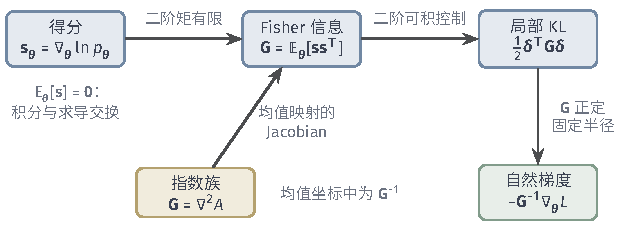
\includegraphics[width=106mm]{figures/07-probability/07-distribution-optimization/tikz/igeo-chain-map/figure.pdf}
  \caption{本章的主线与各步条件。蓝框依次为得分、Fisher信息与局部KL，箭头旁是由前一项得到后一项所需的条件；绿框为自然梯度，需要$\bm{G}$正定；黄框为指数族，其中Fisher信息是对数配分函数的Hessian，也是均值映射的Jacobian。}
  \label{fig:igeo-chain-map}
\end{BookInlineFigure}

正则分布族是这条链的起点：参数集合是开集，支撑不随参数移动，密度对参数可微，并且求导能与积分交换。在这些条件下，得分的期望为零，这是总质量守恒的表现；支撑随参数移动的模型（如$\operatorname{Unif}(0,\theta)$）会多出边界项，KL散度甚至可能为无穷，本章的结论不适用于它们。Fisher信息总是半正定的，但不一定正定。参数冗余、某点的一阶退化与整体不可辨识是三件不同的事，凡要求逆，都要先排除前两种情形。

KL散度的二阶展开说明Fisher信息就是分布变化的局部尺度，系数$\frac12$对应自然对数。它只在一点附近成立：位移稍大，两个方向的KL散度就明显分开，也可能因为整体不可辨识而降到零。换参数坐标时，Fisher信息按$\bm{J}^{\top}\bm{G}\bm{J}$变换，切向量的二次型保持不变。表~\ref{tab:igeo-summary}汇总了高斯族在几套坐标下的结果。

\begin{BookInlineTable}
  \centering
  \caption{高斯族$\mathcal{N}(\mu,\sigma^{2})$在不同坐标下的Fisher信息，$v=\sigma^{2}$，$\tau=\ln v$。各行表示同一个分布族，局部变化的二次型相同。}
  \label{tab:igeo-summary}
  \begin{tabular}{lll}
    \toprule
    坐标 & Fisher信息 & 特点 \\
    \midrule
    $(\mu,\sigma)$ & $\operatorname{diag}(1/\sigma^{2},\,2/\sigma^{2})$ & 尺度随$\sigma$缩小而增大 \\
    $(\mu,v)$ & $\operatorname{diag}(1/v,\,1/(2v^{2}))$ & 方差方向随$v$增大变得便宜 \\
    $(\mu,\tau)$ & $\operatorname{diag}(1/v,\,1/2)$ & 方差方向的尺度处处相同 \\
    自然参数 & $\operatorname{Cov}(X,X^{2})$ & 非对角，等于$\nabla^{2}A$ \\
    均值参数 & 自然参数下信息的逆 & 与自然参数对偶 \\
    \bottomrule
  \end{tabular}
\end{BookInlineTable}

指数族把这些结构集中到对数配分函数上：得分是自然统计量减去均值，Fisher信息是$\nabla^{2}A$，KL散度是由$A$生成的Bregman距离。均值映射的Jacobian就是Fisher信息，所以均值坐标下的Fisher信息是它的逆；对偶势函数$A^{*}$在均值坐标中扮演$A$的角色。这些对应只在最小表示的正则指数族内部成立，冗余统计量与边界参数都会使它失效。

自然梯度是在固定的局部KL预算下使目标一阶下降最多的方向，要求Fisher信息正定、梯度非零。它在坐标变换下表示同一个切向量，普通梯度没有这个性质；但有限步更新还依赖步长和回到参数空间的规则，不同坐标中相加同一个方向，一般得到不同的新分布。实施时，方向由解线性方程得到，信息矩阵可能需要用候选分布自身的样本估计，大规模时只用Fisher向量积近似求解；步长要同时受局部预算、可行性与实际下降的约束。局部几何只回答“朝哪里走、一步走多远才算小”，全局收敛、估计精度与族内逼近误差都需要另外检验。

Fisher信息还出现在统计估计中：它给出由样本估计参数时精度的下界。那是在给定数据下讨论估计量的性质，属于统计推断的问题，可参考\BookChapterRef{chap:finite-sample-lower-bounds}{卷八第5章“有限样本的精度下界”}。
